\documentclass[]{article}
\usepackage{lmodern}
\usepackage{amssymb,amsmath}
\usepackage{ifxetex,ifluatex}
\usepackage{fixltx2e} % provides \textsubscript
\ifnum 0\ifxetex 1\fi\ifluatex 1\fi=0 % if pdftex
  \usepackage[T1]{fontenc}
  \usepackage[utf8]{inputenc}
\else % if luatex or xelatex
  \ifxetex
    \usepackage{mathspec}
  \else
    \usepackage{fontspec}
  \fi
  \defaultfontfeatures{Ligatures=TeX,Scale=MatchLowercase}
\fi
% use upquote if available, for straight quotes in verbatim environments
\IfFileExists{upquote.sty}{\usepackage{upquote}}{}
% use microtype if available
\IfFileExists{microtype.sty}{%
\usepackage{microtype}
\UseMicrotypeSet[protrusion]{basicmath} % disable protrusion for tt fonts
}{}
\usepackage[margin=1in]{geometry}
\usepackage{hyperref}
\hypersetup{unicode=true,
            pdftitle={Final Project - Yelp Recommender System},
            pdfauthor={Juliann McEachern, Rajwant Mishra,Christina Valore},
            pdfborder={0 0 0},
            breaklinks=true}
\urlstyle{same}  % don't use monospace font for urls
\usepackage{color}
\usepackage{fancyvrb}
\newcommand{\VerbBar}{|}
\newcommand{\VERB}{\Verb[commandchars=\\\{\}]}
\DefineVerbatimEnvironment{Highlighting}{Verbatim}{commandchars=\\\{\}}
% Add ',fontsize=\small' for more characters per line
\usepackage{framed}
\definecolor{shadecolor}{RGB}{248,248,248}
\newenvironment{Shaded}{\begin{snugshade}}{\end{snugshade}}
\newcommand{\AlertTok}[1]{\textcolor[rgb]{0.94,0.16,0.16}{#1}}
\newcommand{\AnnotationTok}[1]{\textcolor[rgb]{0.56,0.35,0.01}{\textbf{\textit{#1}}}}
\newcommand{\AttributeTok}[1]{\textcolor[rgb]{0.77,0.63,0.00}{#1}}
\newcommand{\BaseNTok}[1]{\textcolor[rgb]{0.00,0.00,0.81}{#1}}
\newcommand{\BuiltInTok}[1]{#1}
\newcommand{\CharTok}[1]{\textcolor[rgb]{0.31,0.60,0.02}{#1}}
\newcommand{\CommentTok}[1]{\textcolor[rgb]{0.56,0.35,0.01}{\textit{#1}}}
\newcommand{\CommentVarTok}[1]{\textcolor[rgb]{0.56,0.35,0.01}{\textbf{\textit{#1}}}}
\newcommand{\ConstantTok}[1]{\textcolor[rgb]{0.00,0.00,0.00}{#1}}
\newcommand{\ControlFlowTok}[1]{\textcolor[rgb]{0.13,0.29,0.53}{\textbf{#1}}}
\newcommand{\DataTypeTok}[1]{\textcolor[rgb]{0.13,0.29,0.53}{#1}}
\newcommand{\DecValTok}[1]{\textcolor[rgb]{0.00,0.00,0.81}{#1}}
\newcommand{\DocumentationTok}[1]{\textcolor[rgb]{0.56,0.35,0.01}{\textbf{\textit{#1}}}}
\newcommand{\ErrorTok}[1]{\textcolor[rgb]{0.64,0.00,0.00}{\textbf{#1}}}
\newcommand{\ExtensionTok}[1]{#1}
\newcommand{\FloatTok}[1]{\textcolor[rgb]{0.00,0.00,0.81}{#1}}
\newcommand{\FunctionTok}[1]{\textcolor[rgb]{0.00,0.00,0.00}{#1}}
\newcommand{\ImportTok}[1]{#1}
\newcommand{\InformationTok}[1]{\textcolor[rgb]{0.56,0.35,0.01}{\textbf{\textit{#1}}}}
\newcommand{\KeywordTok}[1]{\textcolor[rgb]{0.13,0.29,0.53}{\textbf{#1}}}
\newcommand{\NormalTok}[1]{#1}
\newcommand{\OperatorTok}[1]{\textcolor[rgb]{0.81,0.36,0.00}{\textbf{#1}}}
\newcommand{\OtherTok}[1]{\textcolor[rgb]{0.56,0.35,0.01}{#1}}
\newcommand{\PreprocessorTok}[1]{\textcolor[rgb]{0.56,0.35,0.01}{\textit{#1}}}
\newcommand{\RegionMarkerTok}[1]{#1}
\newcommand{\SpecialCharTok}[1]{\textcolor[rgb]{0.00,0.00,0.00}{#1}}
\newcommand{\SpecialStringTok}[1]{\textcolor[rgb]{0.31,0.60,0.02}{#1}}
\newcommand{\StringTok}[1]{\textcolor[rgb]{0.31,0.60,0.02}{#1}}
\newcommand{\VariableTok}[1]{\textcolor[rgb]{0.00,0.00,0.00}{#1}}
\newcommand{\VerbatimStringTok}[1]{\textcolor[rgb]{0.31,0.60,0.02}{#1}}
\newcommand{\WarningTok}[1]{\textcolor[rgb]{0.56,0.35,0.01}{\textbf{\textit{#1}}}}
\usepackage{graphicx,grffile}
\makeatletter
\def\maxwidth{\ifdim\Gin@nat@width>\linewidth\linewidth\else\Gin@nat@width\fi}
\def\maxheight{\ifdim\Gin@nat@height>\textheight\textheight\else\Gin@nat@height\fi}
\makeatother
% Scale images if necessary, so that they will not overflow the page
% margins by default, and it is still possible to overwrite the defaults
% using explicit options in \includegraphics[width, height, ...]{}
\setkeys{Gin}{width=\maxwidth,height=\maxheight,keepaspectratio}
\IfFileExists{parskip.sty}{%
\usepackage{parskip}
}{% else
\setlength{\parindent}{0pt}
\setlength{\parskip}{6pt plus 2pt minus 1pt}
}
\setlength{\emergencystretch}{3em}  % prevent overfull lines
\providecommand{\tightlist}{%
  \setlength{\itemsep}{0pt}\setlength{\parskip}{0pt}}
\setcounter{secnumdepth}{0}
% Redefines (sub)paragraphs to behave more like sections
\ifx\paragraph\undefined\else
\let\oldparagraph\paragraph
\renewcommand{\paragraph}[1]{\oldparagraph{#1}\mbox{}}
\fi
\ifx\subparagraph\undefined\else
\let\oldsubparagraph\subparagraph
\renewcommand{\subparagraph}[1]{\oldsubparagraph{#1}\mbox{}}
\fi

%%% Use protect on footnotes to avoid problems with footnotes in titles
\let\rmarkdownfootnote\footnote%
\def\footnote{\protect\rmarkdownfootnote}

%%% Change title format to be more compact
\usepackage{titling}

% Create subtitle command for use in maketitle
\providecommand{\subtitle}[1]{
  \posttitle{
    \begin{center}\large#1\end{center}
    }
}

\setlength{\droptitle}{-2em}

  \title{Final Project - Yelp Recommender System}
    \pretitle{\vspace{\droptitle}\centering\huge}
  \posttitle{\par}
    \author{Juliann McEachern, Rajwant Mishra,Christina Valore}
    \preauthor{\centering\large\emph}
  \postauthor{\par}
      \predate{\centering\large\emph}
  \postdate{\par}
    \date{July 16, 2019}

\usepackage{booktabs}
\usepackage{longtable}
\usepackage{array}
\usepackage{multirow}
\usepackage{wrapfig}
\usepackage{float}
\usepackage{colortbl}
\usepackage{pdflscape}
\usepackage{tabu}
\usepackage{threeparttable}
\usepackage{threeparttablex}
\usepackage[normalem]{ulem}
\usepackage{makecell}
\usepackage{xcolor}

\begin{document}
\maketitle

{
\setcounter{tocdepth}{2}
\tableofcontents
}
\hypertarget{overview}{%
\section{Overview}\label{overview}}

Our project used data from Kaggle's 2013 Yelp Challenge. This challenge
included a subset of Yelp data from the metropolitan area of Phoenix,
Arizona. Our data takes into account user reviews, ratings, and check-in
data for a wide-range of businesses.

\hypertarget{data-aquisition-transformations}{%
\subsection{Data Aquisition \&
Transformations}\label{data-aquisition-transformations}}

Data was acquired and transformed in the \texttt{preprocessing.R} file
located within our repositories final-project folder. Our data source
was provided as multiarray Json files, meaning each file is a collection
of json data. We used \texttt{stream\_in} function, which parses json
data line-by-line from the data folder of our repository. The
collections included three, large data for Yelp businesses, users, and
reviews.

Once obtained, we prepared our data for our recommender system using the
following transformations:

\hypertarget{business}{%
\subsubsection{Business}\label{business}}

We choose to limit the scope to our recommender system to only
businesses with tags related to food and beverages. There were
originally 508 unique category tags listed within our business data. We
manually filtered 112 targeted categories to subset our data.

We applied additional transformation to remove unnessacary data. There
were 1,224 business in our data that were permanently closed. These
companies accounted for 9.8\% of all businesses, which were subsequently
removed from our data. There were also 3 businesses in our dataset from
outside of AZ that we also removed.

As a result of our transformations, our recommender data was shortened
4,828 unique businesses. This was further limited to 4,332 after
randomly sampling our user-data. The output of which can be previewed
below:

\begin{table}[t]

\caption{\label{tab:business}Preview Business Data}
\centering
\fontsize{10}{12}\selectfont
\begin{tabu} to \linewidth {>{\raggedright}X>{\raggedright}X>{\raggedright}X>{\raggedright}X>{\raggedleft}X>{\raggedright}X>{\raggedleft}X}
\hline
business\_id & categories & city & name & longitude & state & latitude\\
\hline
usAsSV36QmUej8--yvN-dg & Food, Grocery & Phoenix & Food City & -112.0854 & AZ & 33.39221\\
\hline
PzOqRohWw7F7YEPBz6AubA & Food, Bagels, Delis, Restaurants & Glendale Az & Hot Bagels \& Deli & -112.2003 & AZ & 33.71280\\
\hline
qarobAbxGSHI7ygf1f7a\_Q & Sandwiches, Restaurants & Gilbert & Jersey Mike's Subs & -111.8120 & AZ & 33.37884\\
\hline
JxVGJ9Nly2FFIs\_WpJvkug & Pizza, Restaurants & Scottsdale & Sauce & -111.9263 & AZ & 33.61746\\
\hline
Jj7bcQ6NDfKoz4TXwvYfMg & Burgers, Restaurants & Phoenix & Fuddruckers & -112.1162 & AZ & 33.56699\\
\hline
JHp5mJvYe6UtM\_QsklR-iw & Pizza, Restaurants & Scottsdale & Peter Piper Pizza & -111.9175 & AZ & 33.46613\\
\hline
\end{tabu}
\end{table}

\hypertarget{review}{%
\subsubsection{Review}\label{review}}

We subset our review data from the subset of food and beverage
businesses. This dropped our review data from 229,907 to 165,823
reviews. We later applied another filter to the data to only use reviews
from 10,000 randomly sampled users. This further decreases reviews to
44,494 observations. Our review data can be previewed in two parts
below:

\begin{table}[t]

\caption{\label{tab:review}Preview Review Data (without Review Text)}
\centering
\fontsize{10}{12}\selectfont
\begin{tabu} to \linewidth {}
\hline
\\
\hline
\end{tabu}
\end{table}

\hypertarget{user}{%
\subsubsection{User}\label{user}}

Next, we applied a similar filter to users to subset our data based on
only our selected businesses. This decreased our user data from 43,873
to 35,268 distinct user\_id observations. Do to processing constraints
in R, we choose to randomly sample 10,000 users from these unique
profiles.

The dataframe preview below shows aggregate user data for all reviews an
individual user provided for yelp within our data selection.

\begin{table}[t]

\caption{\label{tab:user}Preview User Data}
\centering
\fontsize{10}{12}\selectfont
\begin{tabu} to \linewidth {>{\raggedright}X>{\raggedright}X>{\raggedleft}X>{\raggedleft}X>{\raggedleft}X>{\raggedleft}X>{\raggedleft}X}
\hline
user\_id & user\_name & review\_count & votes.funny & votes.useful & votes.cool & average\_stars\\
\hline
--lMCM6K8-9NTvPlbCMXEA & Anne Marie & 1 & 0 & 0 & 0 & 4.0\\
\hline
--LzFD0UDbYE-Oho3AhsOg & Shumai & 1 & 0 & 1 & 0 & 4.0\\
\hline
--M-cIkGnH1KhnLaCOmoPQ & Emma & 1 & 2 & 2 & 2 & 5.0\\
\hline
-01H9S7YxFrhRgNdvxmaVQ & Marc & 1 & 0 & 0 & 0 & 5.0\\
\hline
-06LYbA4Qm\_9E83KNT1Jrg & Brett & 2 & 0 & 0 & 0 & 4.5\\
\hline
-0Ycl6yN0BsX1U70-SZOYw & Kate & 2 & 0 & 0 & 0 & 4.0\\
\hline
\end{tabu}
\end{table}

\hypertarget{merged-dataframe}{%
\subsubsection{Merged Dataframe}\label{merged-dataframe}}

Last, we created our main dataframe by merging business and reviews on
\texttt{Business\_ID}. This dataframe will serve as the source of data
for our recommender algorithms. The user and business unique keys were
simplified from characters to numeric user/item identifiers.

This dataframe will be referenced later on when building our recommender
matrices and algorithms.

\begin{table}[t]

\caption{\label{tab:df}Preview main dataframe}
\centering
\fontsize{10}{12}\selectfont
\begin{tabu} to \linewidth {>{\raggedright}X>{\raggedright}X>{\raggedright}X>{\raggedleft}X>{\raggedright}X>{\raggedleft}X>{\raggedleft}X>{\raggedleft}X>{\raggedleft}X>{\raggedleft}X>{\raggedright}X>{\raggedleft}X>{\raggedleft}X}
\hline
categories & city & name & longitude & state & latitude & votes.funny & votes.useful & votes.cool & stars & date & userID & itemID\\
\hline
Food, Grocery & Phoenix & Food City & -112.0854 & AZ & 33.39221 & 0 & 0 & 0 & 3 & 2011-11-20 & 1 & 1\\
\hline
Food, Bagels, Delis, Restaurants & Glendale Az & Hot Bagels \& Deli & -112.2003 & AZ & 33.71280 & 0 & 1 & 0 & 4 & 2012-06-11 & 2 & 2\\
\hline
Sandwiches, Restaurants & Gilbert & Jersey Mike's Subs & -111.8120 & AZ & 33.37884 & 1 & 0 & 0 & 2 & 2012-08-27 & 3 & 3\\
\hline
Sandwiches, Restaurants & Gilbert & Jersey Mike's Subs & -111.8120 & AZ & 33.37884 & 0 & 1 & 0 & 3 & 2012-03-09 & 4 & 3\\
\hline
Sandwiches, Restaurants & Gilbert & Jersey Mike's Subs & -111.8120 & AZ & 33.37884 & 1 & 2 & 1 & 4 & 2012-05-10 & 5 & 3\\
\hline
Pizza, Restaurants & Scottsdale & Sauce & -111.9263 & AZ & 33.61746 & 0 & 0 & 0 & 5 & 2011-09-22 & 6 & 4\\
\hline
\end{tabu}
\end{table}

\hypertarget{recommender-algorithms}{%
\section{Recommender Algorithms}\label{recommender-algorithms}}

We tested recommender algorithms using \texttt{recommenderlab} and
\texttt{sparklyr} to see which performed the best on our recommender
system data. To test the algorithsm, we first had to create a user-item
matrix and then split our data into training and test sets.

\hypertarget{realratingsmatrix}{%
\subsection{RealRatingsMatrix}\label{realratingsmatrix}}

\hypertarget{matrix-building}{%
\subsubsection{Matrix Building}\label{matrix-building}}

We converted our raw ratings data into a user-item matrix to test and
train our subsequent recommender system algorithms. The matrix was saved
as a realRatingMatrix for processing purposes later on using the
\texttt{recommenderlab} package.

\begin{Shaded}
\begin{Highlighting}[]
\CommentTok{# spread data from long to wide format}
\NormalTok{matrix_data <-}\StringTok{ }\NormalTok{df }\OperatorTok\StringTok{ }\KeywordTok{select}\NormalTok{(userID, itemID, stars) }\OperatorTok\StringTok{ }\KeywordTok{spread}\NormalTok{(itemID, stars)}
\CommentTok{# set row names to userid}
\KeywordTok{rownames}\NormalTok{(matrix_data) <-}\StringTok{ }\NormalTok{matrix_data}\OperatorTok{$}\NormalTok{userID}
\CommentTok{# remove userid from columns}
\NormalTok{matrix_data <-}\StringTok{ }\NormalTok{matrix_data }\OperatorTok\StringTok{ }\KeywordTok{select}\NormalTok{(}\OperatorTok{-}\NormalTok{userID)}
\CommentTok{# convert to matrix}
\NormalTok{ui_mat <-}\StringTok{ }\NormalTok{matrix_data }\OperatorTok\StringTok{ }\KeywordTok{as.matrix}\NormalTok{()}
\CommentTok{# store matrix as realRatingMatrix}
\NormalTok{ui_mat <-}\StringTok{ }\KeywordTok{as}\NormalTok{(ui_mat, }\StringTok{"realRatingMatrix"}\NormalTok{)}
\end{Highlighting}
\end{Shaded}

\begin{verbatim}
FALSE    1  2  3  4  5  6  7  8  9 10 11 12 13 14 15 16 17 18 19 20 21 22 23 24
FALSE   25 26 27 28 29 30 31 32 33 34 35 36 37 38 39 40 41 42 43 44 45 46 47 48
FALSE   49 50 51 52 53 54 55 56 57 58 59 60 61 62 63 64 65 66 67 68 69 70 71 72
FALSE   73 74 75 76 77 78 79 80 81 82 83 84 85 86 87 88 89 90 91 92 93 94 95 96
FALSE   97 98 99 100 101 102 103 104 105 106 107 108 109 110 111 112 113 114 115
FALSE   116 117 118 119 120 121 122 123 124 125 126 127 128 129 130 131 132 133
FALSE   134 135 136 137 138 139 140 141 142 143 144 145 146 147 148 149 150 151
FALSE   152 153 154 155 156 157 158 159 160 161 162 163 164 165 166 167 168 169
FALSE   170 171 172 173 174 175 176 177 178 179 180 181 182 183 184 185 186 187
FALSE   188 189 190 191 192 193 194 195 196 197 198 199 200 201 202 203 204 205
FALSE   206 207 208 209 210 211 212 213 214 215 216 217 218 219 220 221 222 223
FALSE   224 225 226 227 228 229 230 231 232 233 234 235 236 237 238 239 240 241
FALSE   242 243 244 245 246 247 248 249 250 251 252 253 254 255 256 257 258 259
FALSE   260 261 262 263 264 265 266 267 268 269 270 271 272 273 274 275 276 277
FALSE   278 279 280 281 282 283 284 285 286 287 288 289 290 291 292 293 294 295
FALSE   296 297 298 299 300 301 302 303 304 305 306 307 308 309 310 311 312 313
FALSE   314 315 316 317 318 319 320 321 322 323 324 325 326 327 328 329 330 331
FALSE   332 333 334 335 336 337 338 339 340 341 342 343 344 345 346 347 348 349
FALSE   350 351 352 353 354 355 356 357 358 359 360 361 362 363 364 365 366 367
FALSE   368 369 370 371 372 373 374 375 376 377 378 379 380 381 382 383 384 385
FALSE   386 387 388 389 390 391 392 393 394 395 396 397 398 399 400 401 402 403
FALSE   404 405 406 407 408 409 410 411 412 413 414 415 416 417 418 419 420 421
FALSE   422 423 424 425 426 427 428 429 430 431 432 433 434 435 436 437 438 439
FALSE   440 441 442 443 444 445 446 447 448 449 450 451 452 453 454 455 456 457
FALSE   458 459 460 461 462 463 464 465 466 467 468 469 470 471 472 473 474 475
FALSE   476 477 478 479 480 481 482 483 484 485 486 487 488 489 490 491 492 493
FALSE   494 495 496 497 498 499 500 501 502 503 504 505 506 507 508 509 510 511
FALSE   512 513 514 515 516 517 518 519 520 521 522 523 524 525 526 527 528 529
FALSE   530 531 532 533 534 535 536 537 538 539 540 541 542 543 544 545 546 547
FALSE   548 549 550 551 552 553 554 555 556 557 558 559 560 561 562 563 564 565
FALSE   566 567 568 569 570 571 572 573 574 575 576 577 578 579 580 581 582 583
FALSE   584 585 586 587 588 589 590 591 592 593 594 595 596 597 598 599 600 601
FALSE   602 603 604 605 606 607 608 609 610 611 612 613 614 615 616 617 618 619
FALSE   620 621 622 623 624 625 626 627 628 629 630 631 632 633 634 635 636 637
FALSE   638 639 640 641 642 643 644 645 646 647 648 649 650 651 652 653 654 655
FALSE   656 657 658 659 660 661 662 663 664 665 666 667 668 669 670 671 672 673
FALSE   674 675 676 677 678 679 680 681 682 683 684 685 686 687 688 689 690 691
FALSE   692 693 694 695 696 697 698 699 700 701 702 703 704 705 706 707 708 709
FALSE   710 711 712 713 714 715 716 717 718 719 720 721 722 723 724 725 726 727
FALSE   728 729 730 731 732 733 734 735 736 737 738 739 740 741 742 743 744 745
FALSE   746 747 748 749 750 751 752 753 754 755 756 757 758 759 760 761 762 763
FALSE   764 765 766 767 768 769 770 771 772 773 774 775 776 777 778 779 780 781
FALSE   782 783 784 785 786 787 788 789 790 791 792 793 794 795 796 797 798 799
FALSE   800 801 802 803 804 805 806 807 808 809 810 811 812 813 814 815 816 817
FALSE   818 819 820 821 822 823 824 825 826 827 828 829 830 831 832 833 834 835
FALSE   836 837 838 839 840 841 842 843 844 845 846 847 848 849 850 851 852 853
FALSE   854 855 856 857 858 859 860 861 862 863 864 865 866 867 868 869 870 871
FALSE   872 873 874 875 876 877 878 879 880 881 882 883 884 885 886 887 888 889
FALSE   890 891 892 893 894 895 896 897 898 899 900 901 902 903 904 905 906 907
FALSE   908 909 910 911 912 913 914 915 916 917 918 919 920 921 922 923 924 925
FALSE   926 927 928 929 930 931 932 933 934 935 936 937 938 939 940 941 942 943
FALSE   944 945 946 947 948 949 950 951 952 953 954 955 956 957 958 959 960 961
FALSE   962 963 964 965 966 967 968 969 970 971 972 973 974 975 976 977 978 979
FALSE   980 981 982 983 984 985 986 987 988 989 990 991 992 993 994 995 996 997
FALSE   998 999 1000 1001 1002 1003 1004 1005 1006 1007 1008 1009 1010 1011 1012
FALSE   1013 1014 1015 1016 1017 1018 1019 1020 1021 1022 1023 1024 1025 1026
FALSE   1027 1028 1029 1030 1031 1032 1033 1034 1035 1036 1037 1038 1039 1040
FALSE   1041 1042 1043 1044 1045 1046 1047 1048 1049 1050 1051 1052 1053 1054
FALSE   1055 1056 1057 1058 1059 1060 1061 1062 1063 1064 1065 1066 1067 1068
FALSE   1069 1070 1071 1072 1073 1074 1075 1076 1077 1078 1079 1080 1081 1082
FALSE   1083 1084 1085 1086 1087 1088 1089 1090 1091 1092 1093 1094 1095 1096
FALSE   1097 1098 1099 1100 1101 1102 1103 1104 1105 1106 1107 1108 1109 1110
FALSE   1111 1112 1113 1114 1115 1116 1117 1118 1119 1120 1121 1122 1123 1124
FALSE   1125 1126 1127 1128 1129 1130 1131 1132 1133 1134 1135 1136 1137 1138
FALSE   1139 1140 1141 1142 1143 1144 1145 1146 1147 1148 1149 1150 1151 1152
FALSE   1153 1154 1155 1156 1157 1158 1159 1160 1161 1162 1163 1164 1165 1166
FALSE   1167 1168 1169 1170 1171 1172 1173 1174 1175 1176 1177 1178 1179 1180
FALSE   1181 1182 1183 1184 1185 1186 1187 1188 1189 1190 1191 1192 1193 1194
FALSE   1195 1196 1197 1198 1199 1200 1201 1202 1203 1204 1205 1206 1207 1208
FALSE   1209 1210 1211 1212 1213 1214 1215 1216 1217 1218 1219 1220 1221 1222
FALSE   1223 1224 1225 1226 1227 1228 1229 1230 1231 1232 1233 1234 1235 1236
FALSE   1237 1238 1239 1240 1241 1242 1243 1244 1245 1246 1247 1248 1249 1250
FALSE   1251 1252 1253 1254 1255 1256 1257 1258 1259 1260 1261 1262 1263 1264
FALSE   1265 1266 1267 1268 1269 1270 1271 1272 1273 1274 1275 1276 1277 1278
FALSE   1279 1280 1281 1282 1283 1284 1285 1286 1287 1288 1289 1290 1291 1292
FALSE   1293 1294 1295 1296 1297 1298 1299 1300 1301 1302 1303 1304 1305 1306
FALSE   1307 1308 1309 1310 1311 1312 1313 1314 1315 1316 1317 1318 1319 1320
FALSE   1321 1322 1323 1324 1325 1326 1327 1328 1329 1330 1331 1332 1333 1334
FALSE   1335 1336 1337 1338 1339 1340 1341 1342 1343 1344 1345 1346 1347 1348
FALSE   1349 1350 1351 1352 1353 1354 1355 1356 1357 1358 1359 1360 1361 1362
FALSE   1363 1364 1365 1366 1367 1368 1369 1370 1371 1372 1373 1374 1375 1376
FALSE   1377 1378 1379 1380 1381 1382 1383 1384 1385 1386 1387 1388 1389 1390
FALSE   1391 1392 1393 1394 1395 1396 1397 1398 1399 1400 1401 1402 1403 1404
FALSE   1405 1406 1407 1408 1409 1410 1411 1412 1413 1414 1415 1416 1417 1418
FALSE   1419 1420 1421 1422 1423 1424 1425 1426 1427 1428 1429 1430 1431 1432
FALSE   1433 1434 1435 1436 1437 1438 1439 1440 1441 1442 1443 1444 1445 1446
FALSE   1447 1448 1449 1450 1451 1452 1453 1454 1455 1456 1457 1458 1459 1460
FALSE   1461 1462 1463 1464 1465 1466 1467 1468 1469 1470 1471 1472 1473 1474
FALSE   1475 1476 1477 1478 1479 1480 1481 1482 1483 1484 1485 1486 1487 1488
FALSE   1489 1490 1491 1492 1493 1494 1495 1496 1497 1498 1499 1500 1501 1502
FALSE   1503 1504 1505 1506 1507 1508 1509 1510 1511 1512 1513 1514 1515 1516
FALSE   1517 1518 1519 1520 1521 1522 1523 1524 1525 1526 1527 1528 1529 1530
FALSE   1531 1532 1533 1534 1535 1536 1537 1538 1539 1540 1541 1542 1543 1544
FALSE   1545 1546 1547 1548 1549 1550 1551 1552 1553 1554 1555 1556 1557 1558
FALSE   1559 1560 1561 1562 1563 1564 1565 1566 1567 1568 1569 1570 1571 1572
FALSE   1573 1574 1575 1576 1577 1578 1579 1580 1581 1582 1583 1584 1585 1586
FALSE   1587 1588 1589 1590 1591 1592 1593 1594 1595 1596 1597 1598 1599 1600
FALSE   1601 1602 1603 1604 1605 1606 1607 1608 1609 1610 1611 1612 1613 1614
FALSE   1615 1616 1617 1618 1619 1620 1621 1622 1623 1624 1625 1626 1627 1628
FALSE   1629 1630 1631 1632 1633 1634 1635 1636 1637 1638 1639 1640 1641 1642
FALSE   1643 1644 1645 1646 1647 1648 1649 1650 1651 1652 1653 1654 1655 1656
FALSE   1657 1658 1659 1660 1661 1662 1663 1664 1665 1666 1667 1668 1669 1670
FALSE   1671 1672 1673 1674 1675 1676 1677 1678 1679 1680 1681 1682 1683 1684
FALSE   1685 1686 1687 1688 1689 1690 1691 1692 1693 1694 1695 1696 1697 1698
FALSE   1699 1700 1701 1702 1703 1704 1705 1706 1707 1708 1709 1710 1711 1712
FALSE   1713 1714 1715 1716 1717 1718 1719 1720 1721 1722 1723 1724 1725 1726
FALSE   1727 1728 1729 1730 1731 1732 1733 1734 1735 1736 1737 1738 1739 1740
FALSE   1741 1742 1743 1744 1745 1746 1747 1748 1749 1750 1751 1752 1753 1754
FALSE   1755 1756 1757 1758 1759 1760 1761 1762 1763 1764 1765 1766 1767 1768
FALSE   1769 1770 1771 1772 1773 1774 1775 1776 1777 1778 1779 1780 1781 1782
FALSE   1783 1784 1785 1786 1787 1788 1789 1790 1791 1792 1793 1794 1795 1796
FALSE   1797 1798 1799 1800 1801 1802 1803 1804 1805 1806 1807 1808 1809 1810
FALSE   1811 1812 1813 1814 1815 1816 1817 1818 1819 1820 1821 1822 1823 1824
FALSE   1825 1826 1827 1828 1829 1830 1831 1832 1833 1834 1835 1836 1837 1838
FALSE   1839 1840 1841 1842 1843 1844 1845 1846 1847 1848 1849 1850 1851 1852
FALSE   1853 1854 1855 1856 1857 1858 1859 1860 1861 1862 1863 1864 1865 1866
FALSE   1867 1868 1869 1870 1871 1872 1873 1874 1875 1876 1877 1878 1879 1880
FALSE   1881 1882 1883 1884 1885 1886 1887 1888 1889 1890 1891 1892 1893 1894
FALSE   1895 1896 1897 1898 1899 1900 1901 1902 1903 1904 1905 1906 1907 1908
FALSE   1909 1910 1911 1912 1913 1914 1915 1916 1917 1918 1919 1920 1921 1922
FALSE   1923 1924 1925 1926 1927 1928 1929 1930 1931 1932 1933 1934 1935 1936
FALSE   1937 1938 1939 1940 1941 1942 1943 1944 1945 1946 1947 1948 1949 1950
FALSE   1951 1952 1953 1954 1955 1956 1957 1958 1959 1960 1961 1962 1963 1964
FALSE   1965 1966 1967 1968 1969 1970 1971 1972 1973 1974 1975 1976 1977 1978
FALSE   1979 1980 1981 1982 1983 1984 1985 1986 1987 1988 1989 1990 1991 1992
FALSE   1993 1994 1995 1996 1997 1998 1999 2000 2001 2002 2003 2004 2005 2006
FALSE   2007 2008 2009 2010 2011 2012 2013 2014 2015 2016 2017 2018 2019 2020
FALSE   2021 2022 2023 2024 2025 2026 2027 2028 2029 2030 2031 2032 2033 2034
FALSE   2035 2036 2037 2038 2039 2040 2041 2042 2043 2044 2045 2046 2047 2048
FALSE   2049 2050 2051 2052 2053 2054 2055 2056 2057 2058 2059 2060 2061 2062
FALSE   2063 2064 2065 2066 2067 2068 2069 2070 2071 2072 2073 2074 2075 2076
FALSE   2077 2078 2079 2080 2081 2082 2083 2084 2085 2086 2087 2088 2089 2090
FALSE   2091 2092 2093 2094 2095 2096 2097 2098 2099 2100 2101 2102 2103 2104
FALSE   2105 2106 2107 2108 2109 2110 2111 2112 2113 2114 2115 2116 2117 2118
FALSE   2119 2120 2121 2122 2123 2124 2125 2126 2127 2128 2129 2130 2131 2132
FALSE   2133 2134 2135 2136 2137 2138 2139 2140 2141 2142 2143 2144 2145 2146
FALSE   2147 2148 2149 2150 2151 2152 2153 2154 2155 2156 2157 2158 2159 2160
FALSE   2161 2162 2163 2164 2165 2166 2167 2168 2169 2170 2171 2172 2173 2174
FALSE   2175 2176 2177 2178 2179 2180 2181 2182 2183 2184 2185 2186 2187 2188
FALSE   2189 2190 2191 2192 2193 2194 2195 2196 2197 2198 2199 2200 2201 2202
FALSE   2203 2204 2205 2206 2207 2208 2209 2210 2211 2212 2213 2214 2215 2216
FALSE   2217 2218 2219 2220 2221 2222 2223 2224 2225 2226 2227 2228 2229 2230
FALSE   2231 2232 2233 2234 2235 2236 2237 2238 2239 2240 2241 2242 2243 2244
FALSE   2245 2246 2247 2248 2249 2250 2251 2252 2253 2254 2255 2256 2257 2258
FALSE   2259 2260 2261 2262 2263 2264 2265 2266 2267 2268 2269 2270 2271 2272
FALSE   2273 2274 2275 2276 2277 2278 2279 2280 2281 2282 2283 2284 2285 2286
FALSE   2287 2288 2289 2290 2291 2292 2293 2294 2295 2296 2297 2298 2299 2300
FALSE   2301 2302 2303 2304 2305 2306 2307 2308 2309 2310 2311 2312 2313 2314
FALSE   2315 2316 2317 2318 2319 2320 2321 2322 2323 2324 2325 2326 2327 2328
FALSE   2329 2330 2331 2332 2333 2334 2335 2336 2337 2338 2339 2340 2341 2342
FALSE   2343 2344 2345 2346 2347 2348 2349 2350 2351 2352 2353 2354 2355 2356
FALSE   2357 2358 2359 2360 2361 2362 2363 2364 2365 2366 2367 2368 2369 2370
FALSE   2371 2372 2373 2374 2375 2376 2377 2378 2379 2380 2381 2382 2383 2384
FALSE   2385 2386 2387 2388 2389 2390 2391 2392 2393 2394 2395 2396 2397 2398
FALSE   2399 2400 2401 2402 2403 2404 2405 2406 2407 2408 2409 2410 2411 2412
FALSE   2413 2414 2415 2416 2417 2418 2419 2420 2421 2422 2423 2424 2425 2426
FALSE   2427 2428 2429 2430 2431 2432 2433 2434 2435 2436 2437 2438 2439 2440
FALSE   2441 2442 2443 2444 2445 2446 2447 2448 2449 2450 2451 2452 2453 2454
FALSE   2455 2456 2457 2458 2459 2460 2461 2462 2463 2464 2465 2466 2467 2468
FALSE   2469 2470 2471 2472 2473 2474 2475 2476 2477 2478 2479 2480 2481 2482
FALSE   2483 2484 2485 2486 2487 2488 2489 2490 2491 2492 2493 2494 2495 2496
FALSE   2497 2498 2499 2500 2501 2502 2503 2504 2505 2506 2507 2508 2509 2510
FALSE   2511 2512 2513 2514 2515 2516 2517 2518 2519 2520 2521 2522 2523 2524
FALSE   2525 2526 2527 2528 2529 2530 2531 2532 2533 2534 2535 2536 2537 2538
FALSE   2539 2540 2541 2542 2543 2544 2545 2546 2547 2548 2549 2550 2551 2552
FALSE   2553 2554 2555 2556 2557 2558 2559 2560 2561 2562 2563 2564 2565 2566
FALSE   2567 2568 2569 2570 2571 2572 2573 2574 2575 2576 2577 2578 2579 2580
FALSE   2581 2582 2583 2584 2585 2586 2587 2588 2589 2590 2591 2592 2593 2594
FALSE   2595 2596 2597 2598 2599 2600 2601 2602 2603 2604 2605 2606 2607 2608
FALSE   2609 2610 2611 2612 2613 2614 2615 2616 2617 2618 2619 2620 2621 2622
FALSE   2623 2624 2625 2626 2627 2628 2629 2630 2631 2632 2633 2634 2635 2636
FALSE   2637 2638 2639 2640 2641 2642 2643 2644 2645 2646 2647 2648 2649 2650
FALSE   2651 2652 2653 2654 2655 2656 2657 2658 2659 2660 2661 2662 2663 2664
FALSE   2665 2666 2667 2668 2669 2670 2671 2672 2673 2674 2675 2676 2677 2678
FALSE   2679 2680 2681 2682 2683 2684 2685 2686 2687 2688 2689 2690 2691 2692
FALSE   2693 2694 2695 2696 2697 2698 2699 2700 2701 2702 2703 2704 2705 2706
FALSE   2707 2708 2709 2710 2711 2712 2713 2714 2715 2716 2717 2718 2719 2720
FALSE   2721 2722 2723 2724 2725 2726 2727 2728 2729 2730 2731 2732 2733 2734
FALSE   2735 2736 2737 2738 2739 2740 2741 2742 2743 2744 2745 2746 2747 2748
FALSE   2749 2750 2751 2752 2753 2754 2755 2756 2757 2758 2759 2760 2761 2762
FALSE   2763 2764 2765 2766 2767 2768 2769 2770 2771 2772 2773 2774 2775 2776
FALSE   2777 2778 2779 2780 2781 2782 2783 2784 2785 2786 2787 2788 2789 2790
FALSE   2791 2792 2793 2794 2795 2796 2797 2798 2799 2800 2801 2802 2803 2804
FALSE   2805 2806 2807 2808 2809 2810 2811 2812 2813 2814 2815 2816 2817 2818
FALSE   2819 2820 2821 2822 2823 2824 2825 2826 2827 2828 2829 2830 2831 2832
FALSE   2833 2834 2835 2836 2837 2838 2839 2840 2841 2842 2843 2844 2845 2846
FALSE   2847 2848 2849 2850 2851 2852 2853 2854 2855 2856 2857 2858 2859 2860
FALSE   2861 2862 2863 2864 2865 2866 2867 2868 2869 2870 2871 2872 2873 2874
FALSE   2875 2876 2877 2878 2879 2880 2881 2882 2883 2884 2885 2886 2887 2888
FALSE   2889 2890 2891 2892 2893 2894 2895 2896 2897 2898 2899 2900 2901 2902
FALSE   2903 2904 2905 2906 2907 2908 2909 2910 2911 2912 2913 2914 2915 2916
FALSE   2917 2918 2919 2920 2921 2922 2923 2924 2925 2926 2927 2928 2929 2930
FALSE   2931 2932 2933 2934 2935 2936 2937 2938 2939 2940 2941 2942 2943 2944
FALSE   2945 2946 2947 2948 2949 2950 2951 2952 2953 2954 2955 2956 2957 2958
FALSE   2959 2960 2961 2962 2963 2964 2965 2966 2967 2968 2969 2970 2971 2972
FALSE   2973 2974 2975 2976 2977 2978 2979 2980 2981 2982 2983 2984 2985 2986
FALSE   2987 2988 2989 2990 2991 2992 2993 2994 2995 2996 2997 2998 2999 3000
FALSE   3001 3002 3003 3004 3005 3006 3007 3008 3009 3010 3011 3012 3013 3014
FALSE   3015 3016 3017 3018 3019 3020 3021 3022 3023 3024 3025 3026 3027 3028
FALSE   3029 3030 3031 3032 3033 3034 3035 3036 3037 3038 3039 3040 3041 3042
FALSE   3043 3044 3045 3046 3047 3048 3049 3050 3051 3052 3053 3054 3055 3056
FALSE   3057 3058 3059 3060 3061 3062 3063 3064 3065 3066 3067 3068 3069 3070
FALSE   3071 3072 3073 3074 3075 3076 3077 3078 3079 3080 3081 3082 3083 3084
FALSE   3085 3086 3087 3088 3089 3090 3091 3092 3093 3094 3095 3096 3097 3098
FALSE   3099 3100 3101 3102 3103 3104 3105 3106 3107 3108 3109 3110 3111 3112
FALSE   3113 3114 3115 3116 3117 3118 3119 3120 3121 3122 3123 3124 3125 3126
FALSE   3127 3128 3129 3130 3131 3132 3133 3134 3135 3136 3137 3138 3139 3140
FALSE   3141 3142 3143 3144 3145 3146 3147 3148 3149 3150 3151 3152 3153 3154
FALSE   3155 3156 3157 3158 3159 3160 3161 3162 3163 3164 3165 3166 3167 3168
FALSE   3169 3170 3171 3172 3173 3174 3175 3176 3177 3178 3179 3180 3181 3182
FALSE   3183 3184 3185 3186 3187 3188 3189 3190 3191 3192 3193 3194 3195 3196
FALSE   3197 3198 3199 3200 3201 3202 3203 3204 3205 3206 3207 3208 3209 3210
FALSE   3211 3212 3213 3214 3215 3216 3217 3218 3219 3220 3221 3222 3223 3224
FALSE   3225 3226 3227 3228 3229 3230 3231 3232 3233 3234 3235 3236 3237 3238
FALSE   3239 3240 3241 3242 3243 3244 3245 3246 3247 3248 3249 3250 3251 3252
FALSE   3253 3254 3255 3256 3257 3258 3259 3260 3261 3262 3263 3264 3265 3266
FALSE   3267 3268 3269 3270 3271 3272 3273 3274 3275 3276 3277 3278 3279 3280
FALSE   3281 3282 3283 3284 3285 3286 3287 3288 3289 3290 3291 3292 3293 3294
FALSE   3295 3296 3297 3298 3299 3300 3301 3302 3303 3304 3305 3306 3307 3308
FALSE   3309 3310 3311 3312 3313 3314 3315 3316 3317 3318 3319 3320 3321 3322
FALSE   3323 3324 3325 3326 3327 3328 3329 3330 3331 3332 3333 3334 3335 3336
FALSE   3337 3338 3339 3340 3341 3342 3343 3344 3345 3346 3347 3348 3349 3350
FALSE   3351 3352 3353 3354 3355 3356 3357 3358 3359 3360 3361 3362 3363 3364
FALSE   3365 3366 3367 3368 3369 3370 3371 3372 3373 3374 3375 3376 3377 3378
FALSE   3379 3380 3381 3382 3383 3384 3385 3386 3387 3388 3389 3390 3391 3392
FALSE   3393 3394 3395 3396 3397 3398 3399 3400 3401 3402 3403 3404 3405 3406
FALSE   3407 3408 3409 3410 3411 3412 3413 3414 3415 3416 3417 3418 3419 3420
FALSE   3421 3422 3423 3424 3425 3426 3427 3428 3429 3430 3431 3432 3433 3434
FALSE   3435 3436 3437 3438 3439 3440 3441 3442 3443 3444 3445 3446 3447 3448
FALSE   3449 3450 3451 3452 3453 3454 3455 3456 3457 3458 3459 3460 3461 3462
FALSE   3463 3464 3465 3466 3467 3468 3469 3470 3471 3472 3473 3474 3475 3476
FALSE   3477 3478 3479 3480 3481 3482 3483 3484 3485 3486 3487 3488 3489 3490
FALSE   3491 3492 3493 3494 3495 3496 3497 3498 3499 3500 3501 3502 3503 3504
FALSE   3505 3506 3507 3508 3509 3510 3511 3512 3513 3514 3515 3516 3517 3518
FALSE   3519 3520 3521 3522 3523 3524 3525 3526 3527 3528 3529 3530 3531 3532
FALSE   3533 3534 3535 3536 3537 3538 3539 3540 3541 3542 3543 3544 3545 3546
FALSE   3547 3548 3549 3550 3551 3552 3553 3554 3555 3556 3557 3558 3559 3560
FALSE   3561 3562 3563 3564 3565 3566 3567 3568 3569 3570 3571 3572 3573 3574
FALSE   3575 3576 3577 3578 3579 3580 3581 3582 3583 3584 3585 3586 3587 3588
FALSE   3589 3590 3591 3592 3593 3594 3595 3596 3597 3598 3599 3600 3601 3602
FALSE   3603 3604 3605 3606 3607 3608 3609 3610 3611 3612 3613 3614 3615 3616
FALSE   3617 3618 3619 3620 3621 3622 3623 3624 3625 3626 3627 3628 3629 3630
FALSE   3631 3632 3633 3634 3635 3636 3637 3638 3639 3640 3641 3642 3643 3644
FALSE   3645 3646 3647 3648 3649 3650 3651 3652 3653 3654 3655 3656 3657 3658
FALSE   3659 3660 3661 3662 3663 3664 3665 3666 3667 3668 3669 3670 3671 3672
FALSE   3673 3674 3675 3676 3677 3678 3679 3680 3681 3682 3683 3684 3685 3686
FALSE   3687 3688 3689 3690 3691 3692 3693 3694 3695 3696 3697 3698 3699 3700
FALSE   3701 3702 3703 3704 3705 3706 3707 3708 3709 3710 3711 3712 3713 3714
FALSE   3715 3716 3717 3718 3719 3720 3721 3722 3723 3724 3725 3726 3727 3728
FALSE   3729 3730 3731 3732 3733 3734 3735 3736 3737 3738 3739 3740 3741 3742
FALSE   3743 3744 3745 3746 3747 3748 3749 3750 3751 3752 3753 3754 3755 3756
FALSE   3757 3758 3759 3760 3761 3762 3763 3764 3765 3766 3767 3768 3769 3770
FALSE   3771 3772 3773 3774 3775 3776 3777 3778 3779 3780 3781 3782 3783 3784
FALSE   3785 3786 3787 3788 3789 3790 3791 3792 3793 3794 3795 3796 3797 3798
FALSE   3799 3800 3801 3802 3803 3804 3805 3806 3807 3808 3809 3810 3811 3812
FALSE   3813 3814 3815 3816 3817 3818 3819 3820 3821 3822 3823 3824 3825 3826
FALSE   3827 3828 3829 3830 3831 3832 3833 3834 3835 3836 3837 3838 3839 3840
FALSE   3841 3842 3843 3844 3845 3846 3847 3848 3849 3850 3851 3852 3853 3854
FALSE   3855 3856 3857 3858 3859 3860 3861 3862 3863 3864 3865 3866 3867 3868
FALSE   3869 3870 3871 3872 3873 3874 3875 3876 3877 3878 3879 3880 3881 3882
FALSE   3883 3884 3885 3886 3887 3888 3889 3890 3891 3892 3893 3894 3895 3896
FALSE   3897 3898 3899 3900 3901 3902 3903 3904 3905 3906 3907 3908 3909 3910
FALSE   3911 3912 3913 3914 3915 3916 3917 3918 3919 3920 3921 3922 3923 3924
FALSE   3925 3926 3927 3928 3929 3930 3931 3932 3933 3934 3935 3936 3937 3938
FALSE   3939 3940 3941 3942 3943 3944 3945 3946 3947 3948 3949 3950 3951 3952
FALSE   3953 3954 3955 3956 3957 3958 3959 3960 3961 3962 3963 3964 3965 3966
FALSE   3967 3968 3969 3970 3971 3972 3973 3974 3975 3976 3977 3978 3979 3980
FALSE   3981 3982 3983 3984 3985 3986 3987 3988 3989 3990 3991 3992 3993 3994
FALSE   3995 3996 3997 3998 3999 4000 4001 4002 4003 4004 4005 4006 4007 4008
FALSE   4009 4010 4011 4012 4013 4014 4015 4016 4017 4018 4019 4020 4021 4022
FALSE   4023 4024 4025 4026 4027 4028 4029 4030 4031 4032 4033 4034 4035 4036
FALSE   4037 4038 4039 4040 4041 4042 4043 4044 4045 4046 4047 4048 4049 4050
FALSE   4051 4052 4053 4054 4055 4056 4057 4058 4059 4060 4061 4062 4063 4064
FALSE   4065 4066 4067 4068 4069 4070 4071 4072 4073 4074 4075 4076 4077 4078
FALSE   4079 4080 4081 4082 4083 4084 4085 4086 4087 4088 4089 4090 4091 4092
FALSE   4093 4094 4095 4096 4097 4098 4099 4100 4101 4102 4103 4104 4105 4106
FALSE   4107 4108 4109 4110 4111 4112 4113 4114 4115 4116 4117 4118 4119 4120
FALSE   4121 4122 4123 4124 4125 4126 4127 4128 4129 4130 4131 4132 4133 4134
FALSE   4135 4136 4137 4138 4139 4140 4141 4142 4143 4144 4145 4146 4147 4148
FALSE   4149 4150 4151 4152 4153 4154 4155 4156 4157 4158 4159 4160 4161 4162
FALSE   4163 4164 4165 4166 4167 4168 4169 4170 4171 4172 4173 4174 4175 4176
FALSE   4177 4178 4179 4180 4181 4182 4183 4184 4185 4186 4187 4188 4189 4190
FALSE   4191 4192 4193 4194 4195 4196 4197 4198 4199 4200 4201 4202 4203 4204
FALSE   4205 4206 4207 4208 4209 4210 4211 4212 4213 4214 4215 4216 4217 4218
FALSE   4219 4220 4221 4222 4223 4224 4225 4226 4227 4228 4229 4230 4231 4232
FALSE   4233 4234 4235 4236 4237 4238 4239 4240 4241 4242 4243 4244 4245 4246
FALSE   4247 4248 4249 4250 4251 4252 4253 4254 4255 4256 4257 4258 4259 4260
FALSE   4261 4262 4263 4264 4265 4266 4267 4268 4269 4270 4271 4272 4273 4274
FALSE   4275 4276 4277 4278 4279 4280 4281 4282 4283 4284 4285 4286 4287 4288
FALSE   4289 4290 4291 4292 4293 4294 4295 4296 4297 4298 4299 4300 4301 4302
FALSE   4303 4304 4305 4306 4307 4308 4309 4310 4311 4312 4313 4314 4315 4316
FALSE   4317 4318 4319 4320 4321 4322 4323 4324 4325 4326 4327 4328 4329 4330
FALSE   4331 4332
FALSE  [ reached getOption("max.print") -- omitted 6 rows ]
\end{verbatim}

\hypertarget{train-and-test-splits}{%
\subsubsection{Train and Test Splits}\label{train-and-test-splits}}

Our data was split into training and tests sets for model evaluation of
both two recommender algorithms. We split our data with 10 k-folds. 80\%
of data was retained for training and 20\% for testing purposes.

\begin{Shaded}
\begin{Highlighting}[]
\CommentTok{# evaluation method with 80% of data for train and 20% for test}
\KeywordTok{set.seed}\NormalTok{(}\DecValTok{0}\NormalTok{)}

\NormalTok{evalu <-}\StringTok{ }\KeywordTok{evaluationScheme}\NormalTok{(ui_mat, }\DataTypeTok{method =} \StringTok{"split"}\NormalTok{, }\DataTypeTok{train =} \FloatTok{0.8}\NormalTok{, }\DataTypeTok{given =} \DecValTok{1}\NormalTok{, }
    \DataTypeTok{goodRating =} \DecValTok{1}\NormalTok{, }\DataTypeTok{k =} \DecValTok{10}\NormalTok{)}

\CommentTok{# prep data}
\NormalTok{train <-}\StringTok{ }\KeywordTok{getData}\NormalTok{(evalu, }\StringTok{"train"}\NormalTok{)  }\CommentTok{# Training Dataset }
\NormalTok{dev_test <-}\StringTok{ }\KeywordTok{getData}\NormalTok{(evalu, }\StringTok{"known"}\NormalTok{)  }\CommentTok{# Test data from evaluationScheme of type KNOWN}
\NormalTok{test <-}\StringTok{ }\KeywordTok{getData}\NormalTok{(evalu, }\StringTok{"unknown"}\NormalTok{)  }\CommentTok{# Unknow datset used for RMSE / model evaluation}
\end{Highlighting}
\end{Shaded}

\hypertarget{user-based-cf}{%
\subsubsection{User-based CF}\label{user-based-cf}}

\begin{Shaded}
\begin{Highlighting}[]
\NormalTok{UB <-}\StringTok{ }\KeywordTok{Recommender}\NormalTok{(}\KeywordTok{getData}\NormalTok{(evalu, }\StringTok{"train"}\NormalTok{), }\StringTok{"UBCF"}\NormalTok{, }\DataTypeTok{param =} \KeywordTok{list}\NormalTok{(}\DataTypeTok{normalize =} \StringTok{"Z-score"}\NormalTok{, }
    \DataTypeTok{method =} \StringTok{"Cosine"}\NormalTok{))}

\NormalTok{p <-}\StringTok{ }\KeywordTok{predict}\NormalTok{(UB, }\KeywordTok{getData}\NormalTok{(evalu, }\StringTok{"known"}\NormalTok{), }\DataTypeTok{type =} \StringTok{"ratings"}\NormalTok{)}

\NormalTok{p}\OperatorTok{@}\NormalTok{data}\OperatorTok{@}\NormalTok{x[p}\OperatorTok{@}\NormalTok{data}\OperatorTok{@}\NormalTok{x[] }\OperatorTok{<}\StringTok{ }\DecValTok{1}\NormalTok{] <-}\StringTok{ }\DecValTok{1}
\NormalTok{p}\OperatorTok{@}\NormalTok{data}\OperatorTok{@}\NormalTok{x[p}\OperatorTok{@}\NormalTok{data}\OperatorTok{@}\NormalTok{x[] }\OperatorTok{>}\StringTok{ }\DecValTok{5}\NormalTok{] <-}\StringTok{ }\DecValTok{5}

\KeywordTok{calcPredictionAccuracy}\NormalTok{(p, }\KeywordTok{getData}\NormalTok{(evalu, }\StringTok{"unknown"}\NormalTok{))}
\end{Highlighting}
\end{Shaded}

\begin{verbatim}
FALSE      RMSE       MSE       MAE 
FALSE 1.3293875 1.7672711 0.9808711
\end{verbatim}

\hypertarget{item-based-cf}{%
\subsubsection{Item-based CF}\label{item-based-cf}}

\begin{Shaded}
\begin{Highlighting}[]
\NormalTok{IB <-}\StringTok{ }\KeywordTok{Recommender}\NormalTok{(}\KeywordTok{getData}\NormalTok{(evalu, }\StringTok{"train"}\NormalTok{), }\StringTok{"IBCF"}\NormalTok{, }\DataTypeTok{param =} \KeywordTok{list}\NormalTok{(}\DataTypeTok{normalize =} \StringTok{"Z-score"}\NormalTok{, }
    \DataTypeTok{method =} \StringTok{"Cosine"}\NormalTok{))}

\NormalTok{p1 <-}\StringTok{ }\KeywordTok{predict}\NormalTok{(IB, }\KeywordTok{getData}\NormalTok{(evalu, }\StringTok{"known"}\NormalTok{), }\DataTypeTok{type =} \StringTok{"ratings"}\NormalTok{)}

\NormalTok{p1}\OperatorTok{@}\NormalTok{data}\OperatorTok{@}\NormalTok{x[p1}\OperatorTok{@}\NormalTok{data}\OperatorTok{@}\NormalTok{x[] }\OperatorTok{<}\StringTok{ }\DecValTok{1}\NormalTok{] <-}\StringTok{ }\DecValTok{1}
\NormalTok{p1}\OperatorTok{@}\NormalTok{data}\OperatorTok{@}\NormalTok{x[p1}\OperatorTok{@}\NormalTok{data}\OperatorTok{@}\NormalTok{x[] }\OperatorTok{>}\StringTok{ }\DecValTok{5}\NormalTok{] <-}\StringTok{ }\DecValTok{5}

\KeywordTok{calcPredictionAccuracy}\NormalTok{(p1, }\KeywordTok{getData}\NormalTok{(evalu, }\StringTok{"unknown"}\NormalTok{))}
\end{Highlighting}
\end{Shaded}

\begin{verbatim}
FALSE     RMSE      MSE      MAE 
FALSE 1.598821 2.556228 1.180108
\end{verbatim}

\hypertarget{binary-ratings-matrix}{%
\subsection{Binary Ratings Matrix}\label{binary-ratings-matrix}}

\begin{itemize}
\tightlist
\item
  In the approach we will work with Bianry dataset and see how Business
  can be Recommended for the Given Business.
\end{itemize}

\hypertarget{binary-rating-matrix}{%
\subsubsection{Binary Rating Matrix}\label{binary-rating-matrix}}

\begin{itemize}
\tightlist
\item
  I first convert the ratings into a binary format to keep things
  simple. ratings of 4 and 5 are
\item
  mapped to 1, representing likes, and ratings of 3 and below are mapped
  to 0, representing dislikes.
\end{itemize}

\begin{Shaded}
\begin{Highlighting}[]
\CommentTok{# Columns are Busienss ID and Row is User_id}
\NormalTok{dat_binaryRatingMatrix <-}\StringTok{ }\NormalTok{df[, }\KeywordTok{c}\NormalTok{(}\DecValTok{11}\NormalTok{, }\DecValTok{1}\NormalTok{, }\DecValTok{13}\NormalTok{)] }\OperatorTok\StringTok{ }\KeywordTok{mutate}\NormalTok{(}\DataTypeTok{Type =} \KeywordTok{case_when}\NormalTok{(stars }\OperatorTok{==}\StringTok{ }
\StringTok{    }\DecValTok{1} \OperatorTok{~}\StringTok{ }\DecValTok{0}\NormalTok{, stars }\OperatorTok{==}\StringTok{ }\DecValTok{2} \OperatorTok{~}\StringTok{ }\DecValTok{0}\NormalTok{, stars }\OperatorTok{==}\StringTok{ }\DecValTok{3} \OperatorTok{~}\StringTok{ }\DecValTok{0}\NormalTok{, stars }\OperatorTok{==}\StringTok{ }\DecValTok{4} \OperatorTok{~}\StringTok{ }\DecValTok{1}\NormalTok{, stars }\OperatorTok{==}\StringTok{ }\DecValTok{5} \OperatorTok{~}\StringTok{ }\DecValTok{1}\NormalTok{, }\OtherTok{TRUE} \OperatorTok{~}\StringTok{ }
\StringTok{    }\DecValTok{0}\NormalTok{)) }\OperatorTok\StringTok{ }\NormalTok{.[}\KeywordTok{c}\NormalTok{(}\DecValTok{1}\NormalTok{, }\DecValTok{2}\NormalTok{, }\DecValTok{4}\NormalTok{)] }\OperatorTok\StringTok{ }\KeywordTok{as}\NormalTok{(}\StringTok{"binaryRatingMatrix"}\NormalTok{)}

\CommentTok{# Creation of Sample dataset. for Evalution Scheme}
\NormalTok{evalu_a2 <-}\StringTok{ }\KeywordTok{evaluationScheme}\NormalTok{(dat_binaryRatingMatrix, }\DataTypeTok{method =} \StringTok{"split"}\NormalTok{, }\DataTypeTok{train =} \FloatTok{0.9}\NormalTok{, }
    \DataTypeTok{given =} \DecValTok{1}\NormalTok{)}

\CommentTok{# Prep data}
\NormalTok{ratings_train <-}\StringTok{ }\KeywordTok{getData}\NormalTok{(evalu_a2, }\StringTok{"train"}\NormalTok{)  }\CommentTok{# Training Dataset }
\NormalTok{ratings_test_known <-}\StringTok{ }\KeywordTok{getData}\NormalTok{(evalu_a2, }\StringTok{"known"}\NormalTok{)  }\CommentTok{# Test data from evaluationScheme of type KNOWN}
\NormalTok{ratings_test_unknown <-}\StringTok{ }\KeywordTok{getData}\NormalTok{(evalu_a2, }\StringTok{"unknown"}\NormalTok{)  }\CommentTok{# Unknow datset used for RMSE / model}

\KeywordTok{head}\NormalTok{(}\KeywordTok{as}\NormalTok{(dat_binaryRatingMatrix[}\DecValTok{1}\OperatorTok{:}\DecValTok{5}\NormalTok{, }\DecValTok{1}\OperatorTok{:}\DecValTok{3}\NormalTok{], }\StringTok{"matrix"}\NormalTok{))}
\end{Highlighting}
\end{Shaded}

\begin{verbatim}
FALSE                        --5jkZ3-nUPZxUvtcbr8Uw --BlvDO_RG2yElKu9XA1_g
FALSE --lMCM6K8-9NTvPlbCMXEA                  FALSE                  FALSE
FALSE --LzFD0UDbYE-Oho3AhsOg                  FALSE                  FALSE
FALSE --M-cIkGnH1KhnLaCOmoPQ                  FALSE                  FALSE
FALSE -01H9S7YxFrhRgNdvxmaVQ                  FALSE                  FALSE
FALSE -06LYbA4Qm_9E83KNT1Jrg                  FALSE                  FALSE
FALSE                        -_JBgygYYD_UkuD-GVTp6A
FALSE --lMCM6K8-9NTvPlbCMXEA                  FALSE
FALSE --LzFD0UDbYE-Oho3AhsOg                  FALSE
FALSE --M-cIkGnH1KhnLaCOmoPQ                  FALSE
FALSE -01H9S7YxFrhRgNdvxmaVQ                  FALSE
FALSE -06LYbA4Qm_9E83KNT1Jrg                  FALSE
\end{verbatim}

\hypertarget{evaluating-the-model}{%
\subsubsection{Evaluating the Model}\label{evaluating-the-model}}

\begin{itemize}
\tightlist
\item
  In this section we are trying to see how ``POPULAR'' method and User
  Based Collaborative Filtering UBCF can recommend the top n items.
\item
  Its also important to note that Binary ratings are not well evaluated
  with the help of Precision and Recall .
\end{itemize}

\begin{Shaded}
\begin{Highlighting}[]
\CommentTok{# creation of recommender model based on ubcf}
\NormalTok{Rec.ubcf <-}\StringTok{ }\KeywordTok{Recommender}\NormalTok{(ratings_train, }\StringTok{"UBCF"}\NormalTok{)}
\CommentTok{# Creating POPULAR recommender model for comparison}
\NormalTok{Rec.pop <-}\StringTok{ }\KeywordTok{Recommender}\NormalTok{(ratings_train, }\StringTok{"POPULAR"}\NormalTok{)}
\CommentTok{# making predictions on the test data set witj Top 2, 3, 5, and 10}
\NormalTok{pred_ubcf2 <-}\StringTok{ }\KeywordTok{predict}\NormalTok{(Rec.ubcf, ratings_test_known, }\DataTypeTok{type =} \StringTok{"topNList"}\NormalTok{, }\DataTypeTok{n =} \DecValTok{2}\NormalTok{)}
\NormalTok{pred_ubcf3 <-}\StringTok{ }\KeywordTok{predict}\NormalTok{(Rec.ubcf, ratings_test_known, }\DataTypeTok{type =} \StringTok{"topNList"}\NormalTok{, }\DataTypeTok{n =} \DecValTok{3}\NormalTok{)}
\NormalTok{pred_ubcf5 <-}\StringTok{ }\KeywordTok{predict}\NormalTok{(Rec.ubcf, ratings_test_known, }\DataTypeTok{type =} \StringTok{"topNList"}\NormalTok{, }\DataTypeTok{n =} \DecValTok{5}\NormalTok{)}
\NormalTok{pred_ubcf10 <-}\StringTok{ }\KeywordTok{predict}\NormalTok{(Rec.ubcf, ratings_test_known, }\DataTypeTok{type =} \StringTok{"topNList"}\NormalTok{, }\DataTypeTok{n =} \DecValTok{10}\NormalTok{)}
\CommentTok{# SAVE IT FOR LATTER USE}
\KeywordTok{saveRDS}\NormalTok{(pred_ubcf2, }\StringTok{"pred_ubcf2.rds"}\NormalTok{)}
\KeywordTok{saveRDS}\NormalTok{(pred_ubcf3, }\StringTok{"pred_ubcf3.rds"}\NormalTok{)}
\KeywordTok{saveRDS}\NormalTok{(pred_ubcf5, }\StringTok{"pred_ubcf5.rds"}\NormalTok{)}
\KeywordTok{saveRDS}\NormalTok{(pred_ubcf10, }\StringTok{"pred_ubcf10.rds"}\NormalTok{)}

\CommentTok{# making predictions on the test data set witj Top 2, 3, 5, and 10}
\NormalTok{pred_pop2 <-}\StringTok{ }\KeywordTok{predict}\NormalTok{(Rec.pop, ratings_test_known, }\DataTypeTok{type =} \StringTok{"topNList"}\NormalTok{, }\DataTypeTok{n =} \DecValTok{2}\NormalTok{)}
\NormalTok{pred_pop3 <-}\StringTok{ }\KeywordTok{predict}\NormalTok{(Rec.pop, ratings_test_known, }\DataTypeTok{type =} \StringTok{"topNList"}\NormalTok{, }\DataTypeTok{n =} \DecValTok{3}\NormalTok{)}
\NormalTok{pred_pop5 <-}\StringTok{ }\KeywordTok{predict}\NormalTok{(Rec.pop, ratings_test_known, }\DataTypeTok{type =} \StringTok{"topNList"}\NormalTok{, }\DataTypeTok{n =} \DecValTok{5}\NormalTok{)}
\NormalTok{pred_pop10 <-}\StringTok{ }\KeywordTok{predict}\NormalTok{(Rec.pop, ratings_test_known, }\DataTypeTok{type =} \StringTok{"topNList"}\NormalTok{, }\DataTypeTok{n =} \DecValTok{10}\NormalTok{)}

\KeywordTok{saveRDS}\NormalTok{(pred_pop2, }\StringTok{"pred_pop2.rds"}\NormalTok{)}
\KeywordTok{saveRDS}\NormalTok{(pred_pop3, }\StringTok{"pred_pop3.rds"}\NormalTok{)}
\KeywordTok{saveRDS}\NormalTok{(pred_pop5, }\StringTok{"pred_pop5.rds"}\NormalTok{)}
\KeywordTok{saveRDS}\NormalTok{(pred_pop10, }\StringTok{"pred_pop10.rds"}\NormalTok{)}


\CommentTok{# Evaluting the Result of UBCF}
\NormalTok{error.ubcf2 <-}\StringTok{ }\KeywordTok{calcPredictionAccuracy}\NormalTok{(pred_ubcf2, ratings_test_unknown, }\DataTypeTok{given =} \DecValTok{0}\NormalTok{)}
\NormalTok{error.ubcf3 <-}\StringTok{ }\KeywordTok{calcPredictionAccuracy}\NormalTok{(pred_ubcf3, ratings_test_unknown, }\DataTypeTok{given =} \DecValTok{0}\NormalTok{)}
\NormalTok{error.ubcf5 <-}\StringTok{ }\KeywordTok{calcPredictionAccuracy}\NormalTok{(pred_ubcf5, ratings_test_unknown, }\DataTypeTok{given =} \DecValTok{0}\NormalTok{)}
\NormalTok{error.ubcf10 <-}\StringTok{ }\KeywordTok{calcPredictionAccuracy}\NormalTok{(pred_ubcf10, ratings_test_unknown, }\DataTypeTok{given =} \DecValTok{0}\NormalTok{)}

\CommentTok{# Evaluting the Result of Popular predictor}
\NormalTok{error.pop2 <-}\StringTok{ }\KeywordTok{calcPredictionAccuracy}\NormalTok{(pred_pop2, ratings_test_unknown, }\DataTypeTok{given =} \DecValTok{0}\NormalTok{)}
\NormalTok{error.pop3 <-}\StringTok{ }\KeywordTok{calcPredictionAccuracy}\NormalTok{(pred_pop3, ratings_test_unknown, }\DataTypeTok{given =} \DecValTok{0}\NormalTok{)}
\NormalTok{error.pop5 <-}\StringTok{ }\KeywordTok{calcPredictionAccuracy}\NormalTok{(pred_pop5, ratings_test_unknown, }\DataTypeTok{given =} \DecValTok{0}\NormalTok{)}
\NormalTok{error.pop10 <-}\StringTok{ }\KeywordTok{calcPredictionAccuracy}\NormalTok{(pred_pop10, ratings_test_unknown, }\DataTypeTok{given =} \DecValTok{0}\NormalTok{)}
\CommentTok{# error.ibcf<-calcPredictionAccuracy(p.ibcf, ratings_test_unknown)}

\NormalTok{error <-}\StringTok{ }\KeywordTok{rbind}\NormalTok{(error.ubcf2, error.ubcf3, error.ubcf5, error.ubcf10, error.pop2, }
\NormalTok{    error.pop3, error.pop5, error.pop10) }\OperatorTok\StringTok{ }\KeywordTok{cbind}\NormalTok{(}\DataTypeTok{TopN =} \KeywordTok{c}\NormalTok{(}\DecValTok{2}\NormalTok{, }\DecValTok{3}\NormalTok{, }\DecValTok{5}\NormalTok{, }\DecValTok{10}\NormalTok{, }\DecValTok{2}\NormalTok{, }
    \DecValTok{3}\NormalTok{, }\DecValTok{5}\NormalTok{, }\DecValTok{10}\NormalTok{), }\DataTypeTok{Type =} \KeywordTok{c}\NormalTok{(}\StringTok{"UBCF"}\NormalTok{, }\StringTok{"UBCF"}\NormalTok{, }\StringTok{"UBCF"}\NormalTok{, }\StringTok{"UBCF"}\NormalTok{, }\StringTok{"POP"}\NormalTok{, }\StringTok{"POP"}\NormalTok{, }\StringTok{"POP"}\NormalTok{, }
    \StringTok{"POP"}\NormalTok{))}
\end{Highlighting}
\end{Shaded}

\textbf{Precision-Recall} Below plot displays the Precesion and Recall
of the POPULAR and UBCF Model, We are looking for higher recall with
maximum precision, and to our surprise POPULAR (Popular items/Business
in our case) MODEL is doing well compare to UBCF. It could be due to the
SAMPLE size.

\begin{Shaded}
\begin{Highlighting}[]
\KeywordTok{as_data_frame}\NormalTok{(error) }\OperatorTok\StringTok{ }\KeywordTok{ggplot}\NormalTok{(}\KeywordTok{aes}\NormalTok{(recall, precision, }\DataTypeTok{color =}\NormalTok{ Type)) }\OperatorTok{+}\StringTok{ }\KeywordTok{geom_line}\NormalTok{() }\OperatorTok{+}\StringTok{ }
\StringTok{    }\KeywordTok{geom_label}\NormalTok{(}\KeywordTok{aes}\NormalTok{(}\DataTypeTok{label =}\NormalTok{ TopN)) }\OperatorTok{+}\StringTok{ }\KeywordTok{labs}\NormalTok{(}\DataTypeTok{title =} \StringTok{"Precision-Recall for Top N"}\NormalTok{, }
    \DataTypeTok{colour =} \StringTok{"Model"}\NormalTok{) }\OperatorTok{+}\StringTok{ }\KeywordTok{theme_grey}\NormalTok{(}\DataTypeTok{base_size =} \DecValTok{14}\NormalTok{) }\OperatorTok{+}\StringTok{ }\KeywordTok{theme}\NormalTok{(}\DataTypeTok{axis.text.x =} \KeywordTok{element_text}\NormalTok{(}\DataTypeTok{angle =} \DecValTok{70}\NormalTok{, }
    \DataTypeTok{hjust =} \DecValTok{1}\NormalTok{))}
\end{Highlighting}
\end{Shaded}

\begin{verbatim}
FALSE Warning: `as_data_frame()` is deprecated, use `as_tibble()` (but mind the new semantics).
FALSE This warning is displayed once per session.
\end{verbatim}

\begin{verbatim}
FALSE geom_path: Each group consists of only one observation. Do you need to
FALSE adjust the group aesthetic?
\end{verbatim}

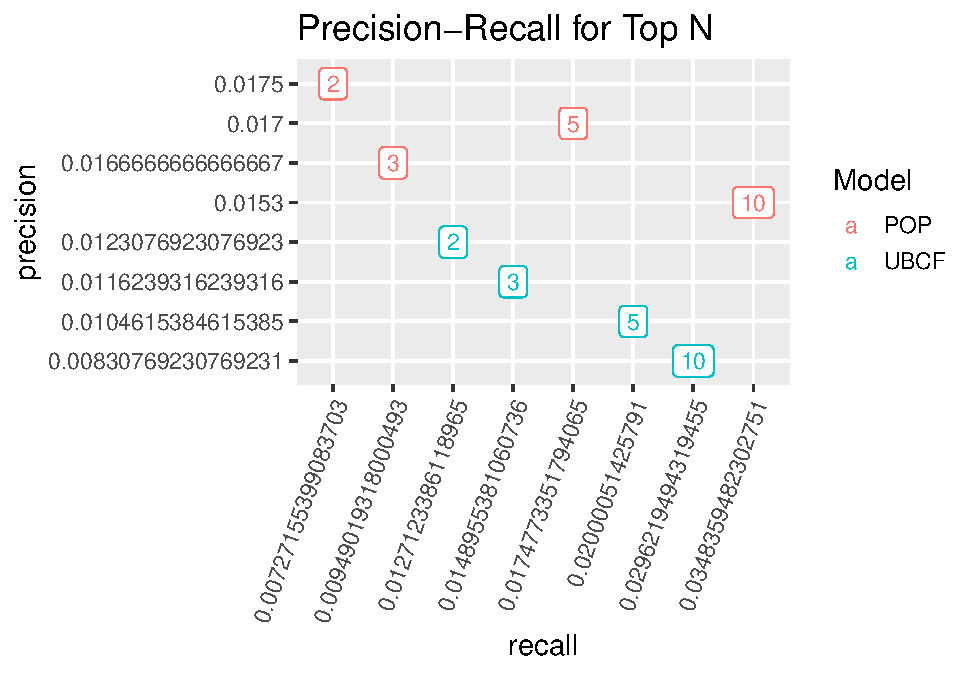
\includegraphics{report_files/figure-latex/unnamed-chunk-3-1.pdf}

** ROC Curve TPR vs FPR** Below Graph is showing the how much is TPR i.e
TRUE Positive (Valid Item/business is getting recommended ,which are
more likely to be visited by users) vs same amount of FPR i.e not a
relevent recommndation . In this case Our focus is to find Max TPR for
any given lvel of FPR.

\begin{Shaded}
\begin{Highlighting}[]
\KeywordTok{as_data_frame}\NormalTok{(error) }\OperatorTok\StringTok{ }\KeywordTok{ggplot}\NormalTok{(}\KeywordTok{aes}\NormalTok{(FPR, TPR, }\DataTypeTok{color =}\NormalTok{ Type)) }\OperatorTok{+}\StringTok{ }\KeywordTok{geom_line}\NormalTok{() }\OperatorTok{+}\StringTok{ }
\StringTok{    }\KeywordTok{geom_label}\NormalTok{(}\KeywordTok{aes}\NormalTok{(}\DataTypeTok{label =}\NormalTok{ TopN)) }\OperatorTok{+}\StringTok{ }\KeywordTok{labs}\NormalTok{(}\DataTypeTok{title =} \StringTok{"ROC Curve / TPR vs FPR"}\NormalTok{, }\DataTypeTok{colour =} \StringTok{"Model"}\NormalTok{) }\OperatorTok{+}\StringTok{ }
\StringTok{    }\KeywordTok{theme_grey}\NormalTok{(}\DataTypeTok{base_size =} \DecValTok{14}\NormalTok{) }\OperatorTok{+}\StringTok{ }\KeywordTok{theme}\NormalTok{(}\DataTypeTok{axis.text.x =} \KeywordTok{element_text}\NormalTok{(}\DataTypeTok{angle =} \DecValTok{70}\NormalTok{, }
    \DataTypeTok{hjust =} \DecValTok{1}\NormalTok{))}
\end{Highlighting}
\end{Shaded}

\begin{verbatim}
FALSE geom_path: Each group consists of only one observation. Do you need to
FALSE adjust the group aesthetic?
\end{verbatim}

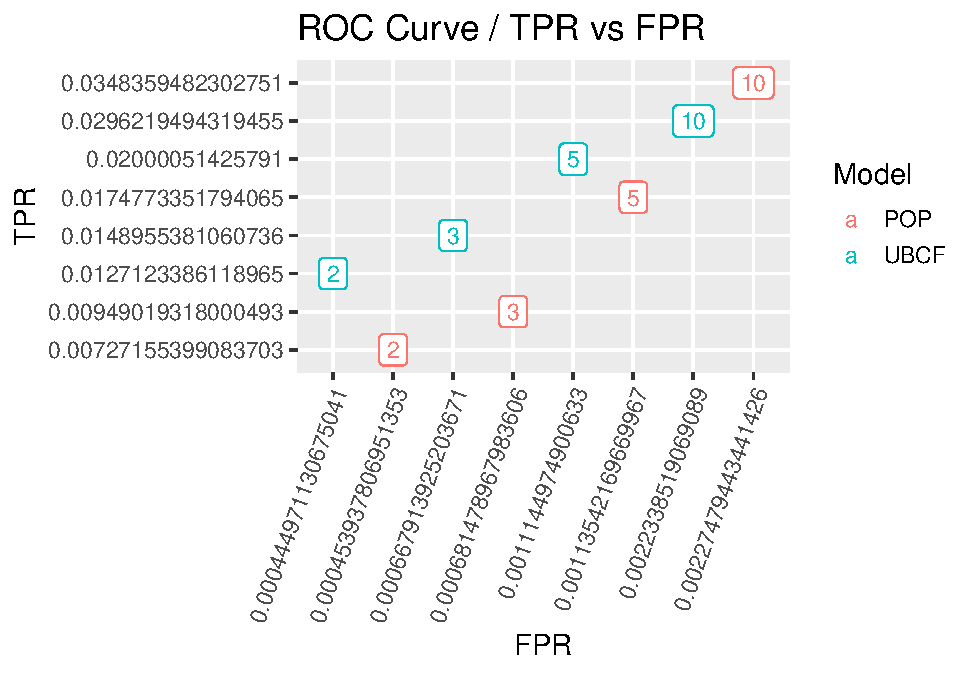
\includegraphics{report_files/figure-latex/unnamed-chunk-4-1.pdf}

\hypertarget{predictions-for-a-new-user}{%
\subsubsection{Predictions For a New
User}\label{predictions-for-a-new-user}}

He we will build the persona of User by visting to a Business
(\texttt{business\_id})

Function to find top 10 Business for the Given Business.

\begin{Shaded}
\begin{Highlighting}[]
\KeywordTok{suppressWarnings}\NormalTok{(}\KeywordTok{REC_TOP_BUSINESS}\NormalTok{(}\StringTok{"SvdlC39JGPI_Tj3pS0ruzw"}\NormalTok{))}
\end{Highlighting}
\end{Shaded}

\begin{verbatim}
FALSE                 business_id
FALSE 1    VVeogjZya58oiTxK7qUjAQ
FALSE 210  JokKtdXU7zXHcr20Lrk29A
FALSE 412  ntN85eu27C04nwyPa8IHtw
FALSE 592  V1nEpIRmEa1768oj_tuxeQ
FALSE 767  EWMwV5V9BxNs_U6nNVMeqw
FALSE 935  WNy1uzcmm_UHmTyR--o5IA
FALSE 1104 -sC66z4SO3tR7nFCjfQwuQ
FALSE 1255 SDwYQ6eSu1htn8vHWv128g
FALSE 1404 QnAzW6KMSciUcuJ20oI3Bw
FALSE 1542 c1yGkETheht_1vjda7G5sA
FALSE                                                                categories
FALSE 1                                                      Pizza, Restaurants
FALSE 210   Bars, Food, Breweries, Pubs, Nightlife, American (New), Restaurants
FALSE 412                                       Breakfast & Brunch, Restaurants
FALSE 592                               Italian, Pizza, Sandwiches, Restaurants
FALSE 767  Bars, Mediterranean, Nightlife, Lounges, American (New), Restaurants
FALSE 935                           Pubs, Bars, Nightlife, British, Restaurants
FALSE 1104                                                 Mexican, Restaurants
FALSE 1255                     Wine Bars, Bars, Restaurants, Nightlife, Italian
FALSE 1404                                  American (Traditional), Restaurants
FALSE 1542                                       Vegetarian, Vegan, Restaurants
FALSE         city                  name
FALSE 1    Phoenix       Pizzeria Bianco
FALSE 210    Tempe Four Peaks Brewing Co
FALSE 412  Phoenix  Matt's Big Breakfast
FALSE 592  Phoenix                  Cibo
FALSE 767  Phoenix                   FEZ
FALSE 935    Tempe Cornish Pasty Company
FALSE 1104 Phoenix     Gallo Blanco Cafe
FALSE 1255 Phoenix       Postino Arcadia
FALSE 1404 Gilbert      Joe's Farm Grill
FALSE 1542   Tempe                 Green
\end{verbatim}

\hypertarget{sparklyr}{%
\subsection{Sparklyr}\label{sparklyr}}

Due to the size of our data, we choose to use Spark in R to avoid
input/output (I/O) bottleneck issues and maximize the performance speed
of our recommender algorithm calculations.

\hypertarget{connecting}{%
\subsubsection{Connecting}\label{connecting}}

We initiated a local connection with Spark (V2.4.3). Our yelp data was
inputted into a spark table and split for training and testing purposes.
We uploaded our training and test splits to minimize the variance in our
comparisons.

\begin{Shaded}
\begin{Highlighting}[]
\CommentTok{# configure spark connection}
\NormalTok{config <-}\StringTok{ }\KeywordTok{spark_config}\NormalTok{()}
\NormalTok{config}\OperatorTok{$}\NormalTok{spark.executor.memory <-}\StringTok{ "8G"}
\NormalTok{config}\OperatorTok{$}\NormalTok{spark.executor.cores <-}\StringTok{ }\DecValTok{2}
\NormalTok{config}\OperatorTok{$}\NormalTok{spark.executor.instances <-}\StringTok{ }\DecValTok{3}
\NormalTok{config}\OperatorTok{$}\NormalTok{spark.dynamicAllocation.enabled <-}\StringTok{ "false"}

\CommentTok{# initiate connection}
\NormalTok{sc <-}\StringTok{ }\KeywordTok{spark_connect}\NormalTok{(}\DataTypeTok{master =} \StringTok{"local"}\NormalTok{, }\DataTypeTok{config =}\NormalTok{ config, }\DataTypeTok{version =} \StringTok{"2.4.3"}\NormalTok{)}

\CommentTok{# unhash to verify version: spark_version(sc)}

\CommentTok{# select data for spark and create spark table}
\NormalTok{spark_train <-}\StringTok{ }\KeywordTok{as}\NormalTok{(train, }\StringTok{"data.frame"}\NormalTok{)}
\NormalTok{spark_test <-}\StringTok{ }\KeywordTok{as}\NormalTok{(test, }\StringTok{"data.frame"}\NormalTok{)}

\NormalTok{spark_train <-}\StringTok{ }\KeywordTok{sdf_copy_to}\NormalTok{(sc, spark_train, }\StringTok{"spark_train"}\NormalTok{, }\DataTypeTok{overwrite =} \OtherTok{TRUE}\NormalTok{)}
\NormalTok{spark_test <-}\StringTok{ }\KeywordTok{sdf_copy_to}\NormalTok{(sc, spark_test, }\StringTok{"spark_test"}\NormalTok{, }\DataTypeTok{overwrite =} \OtherTok{TRUE}\NormalTok{)}

\CommentTok{# Transform features}
\NormalTok{spark_train <-}\StringTok{ }\NormalTok{spark_train }\OperatorTok\StringTok{ }\KeywordTok{ft_string_indexer}\NormalTok{(}\DataTypeTok{input_col =} \StringTok{"user"}\NormalTok{, }\DataTypeTok{output_col =} \StringTok{"user_index"}\NormalTok{) }\OperatorTok\StringTok{ }
\StringTok{    }\KeywordTok{ft_string_indexer}\NormalTok{(}\DataTypeTok{input_col =} \StringTok{"item"}\NormalTok{, }\DataTypeTok{output_col =} \StringTok{"item_index"}\NormalTok{) }\OperatorTok\StringTok{ }\KeywordTok{sdf_register}\NormalTok{(}\StringTok{"spark_train"}\NormalTok{)}

\NormalTok{spark_test <-}\StringTok{ }\NormalTok{spark_test }\OperatorTok\StringTok{ }\KeywordTok{ft_string_indexer}\NormalTok{(}\DataTypeTok{input_col =} \StringTok{"user"}\NormalTok{, }\DataTypeTok{output_col =} \StringTok{"user_index"}\NormalTok{) }\OperatorTok\StringTok{ }
\StringTok{    }\KeywordTok{ft_string_indexer}\NormalTok{(}\DataTypeTok{input_col =} \StringTok{"item"}\NormalTok{, }\DataTypeTok{output_col =} \StringTok{"item_index"}\NormalTok{) }\OperatorTok\StringTok{ }\KeywordTok{sdf_register}\NormalTok{(}\StringTok{"spark_test"}\NormalTok{)}
\end{Highlighting}
\end{Shaded}

\hypertarget{als}{%
\subsubsection{ALS}\label{als}}

Once connected, we applied the alternating least squares (ALS) for our
recommender predictions.

\begin{Shaded}
\begin{Highlighting}[]
\CommentTok{# build model using user/business/ratings}
\NormalTok{als_fit <-}\StringTok{ }\KeywordTok{ml_als}\NormalTok{(spark_train, }\DataTypeTok{max_iter =} \DecValTok{5}\NormalTok{, }\DataTypeTok{nonnegative =} \OtherTok{TRUE}\NormalTok{, }\DataTypeTok{rating_col =} \StringTok{"rating"}\NormalTok{, }
    \DataTypeTok{user_col =} \StringTok{"user_index"}\NormalTok{, }\DataTypeTok{item_col =} \StringTok{"item_index"}\NormalTok{)}

\CommentTok{# predict from the model for the training data}
\NormalTok{als_predict_train <-}\StringTok{ }\KeywordTok{ml_predict}\NormalTok{(als_fit, spark_train) }\OperatorTok\StringTok{ }\KeywordTok{collect}\NormalTok{()}
\NormalTok{als_predict_test <-}\StringTok{ }\KeywordTok{ml_predict}\NormalTok{(als_fit, spark_test) }\OperatorTok\StringTok{ }\KeywordTok{collect}\NormalTok{()}

\CommentTok{# Remove NaN (result of test/train splits - not data)}
\NormalTok{als_predict_train <-}\StringTok{ }\NormalTok{als_predict_train[}\OperatorTok{!}\KeywordTok{is.na}\NormalTok{(als_predict_train}\OperatorTok{$}\NormalTok{prediction), }
\NormalTok{    ]}
\NormalTok{als_predict_test <-}\StringTok{ }\NormalTok{als_predict_test[}\OperatorTok{!}\KeywordTok{is.na}\NormalTok{(als_predict_test}\OperatorTok{$}\NormalTok{prediction), ]}

\CommentTok{# Set floor/ceiling for predictions}
\NormalTok{als_predict_train}\OperatorTok{$}\NormalTok{prediction[als_predict_train}\OperatorTok{$}\NormalTok{prediction }\OperatorTok{<}\StringTok{ }\DecValTok{1}\NormalTok{] <-}\StringTok{ }\DecValTok{1}
\NormalTok{als_predict_train}\OperatorTok{$}\NormalTok{prediction[als_predict_train}\OperatorTok{$}\NormalTok{prediction }\OperatorTok{>}\StringTok{ }\DecValTok{5}\NormalTok{] <-}\StringTok{ }\DecValTok{5}
\NormalTok{als_predict_test}\OperatorTok{$}\NormalTok{prediction[als_predict_test}\OperatorTok{$}\NormalTok{prediction }\OperatorTok{<}\StringTok{ }\DecValTok{1}\NormalTok{] <-}\StringTok{ }\DecValTok{1}
\NormalTok{als_predict_test}\OperatorTok{$}\NormalTok{prediction[als_predict_test}\OperatorTok{$}\NormalTok{prediction }\OperatorTok{>}\StringTok{ }\DecValTok{5}\NormalTok{] <-}\StringTok{ }\DecValTok{5}

\CommentTok{# View results}
\NormalTok{als_predict_test }\OperatorTok\StringTok{ }\KeywordTok{head}\NormalTok{() }\OperatorTok\StringTok{ }\KeywordTok{kable}\NormalTok{() }\OperatorTok\StringTok{ }\KeywordTok{kable_styling}\NormalTok{()}
\end{Highlighting}
\end{Shaded}

\begingroup\fontsize{10}{12}\selectfont

\begin{tabu} to \linewidth {>{\raggedright}X>{\raggedright}X>{\raggedleft}X>{\raggedleft}X>{\raggedleft}X>{\raggedleft}X}
\hline
user & item & rating & user\_index & item\_index & prediction\\
\hline
1748 & 3339 & 5 & 93 & 12 & 3.827803\\
\hline
3905 & 3339 & 4 & 107 & 12 & 3.893977\\
\hline
3052 & 3339 & 2 & 171 & 12 & 4.387575\\
\hline
3691 & 3339 & 4 & 105 & 12 & 3.886786\\
\hline
2549 & 3339 & 5 & 311 & 12 & 2.878149\\
\hline
639 & 3339 & 3 & 10 & 12 & 4.169810\\
\hline
\end{tabu}
\endgroup{}

\hypertarget{performance}{%
\subsubsection{Performance}\label{performance}}

Our ALS calculations for RMSE, MSE, and MAE can be viewed below:

\begin{Shaded}
\begin{Highlighting}[]
\CommentTok{# Calculate RMSE/MSE/MAE}
\NormalTok{als_mse_train <-}\StringTok{ }\KeywordTok{mean}\NormalTok{((als_predict_train}\OperatorTok{$}\NormalTok{rating }\OperatorTok{-}\StringTok{ }\NormalTok{als_predict_train}\OperatorTok{$}\NormalTok{prediction)}\OperatorTok{^}\DecValTok{2}\NormalTok{)}
\NormalTok{als_rmse_train <-}\StringTok{ }\KeywordTok{sqrt}\NormalTok{(als_mse_train)}
\NormalTok{als_mae_train <-}\StringTok{ }\KeywordTok{mean}\NormalTok{(}\KeywordTok{abs}\NormalTok{(als_predict_train}\OperatorTok{$}\NormalTok{rating }\OperatorTok{-}\StringTok{ }\NormalTok{als_predict_train}\OperatorTok{$}\NormalTok{prediction))}

\NormalTok{als_mse_test <-}\StringTok{ }\KeywordTok{mean}\NormalTok{((als_predict_test}\OperatorTok{$}\NormalTok{rating }\OperatorTok{-}\StringTok{ }\NormalTok{als_predict_test}\OperatorTok{$}\NormalTok{prediction)}\OperatorTok{^}\DecValTok{2}\NormalTok{)}
\NormalTok{als_rmse_test <-}\StringTok{ }\KeywordTok{sqrt}\NormalTok{(als_mse_test)}
\NormalTok{als_mae_test <-}\StringTok{ }\KeywordTok{mean}\NormalTok{(}\KeywordTok{abs}\NormalTok{(als_predict_test}\OperatorTok{$}\NormalTok{rating }\OperatorTok{-}\StringTok{ }\NormalTok{als_predict_test}\OperatorTok{$}\NormalTok{prediction))}
\end{Highlighting}
\end{Shaded}

\begin{table}[t]

\caption{\label{tab:view-als}ALS Performance}
\centering
\fontsize{10}{12}\selectfont
\begin{tabu} to \linewidth {>{\raggedright}X>{\raggedleft}X>{\raggedleft}X>{\raggedleft}X}
\hline
type & rmse & mse & mae\\
\hline
ALS\_train & 0.3776714 & 0.1426357 & 0.2595885\\
\hline
ALS\_test & 1.3790567 & 1.9017975 & 1.1070010\\
\hline
\end{tabu}
\end{table}

\hypertarget{recommend}{%
\subsubsection{Recommend}\label{recommend}}

The \texttt{ml\_recommend} function allows us to see the top \emph{n}
user/item recommendations for each user/item. Below, we use this funcion
and filtered our recommendations to show the top 10 restaurant
recommendations for a selected user.

\begin{Shaded}
\begin{Highlighting}[]
\NormalTok{als_user_recommend <-}\StringTok{ }\KeywordTok{ml_recommend}\NormalTok{(als_fit, }\DataTypeTok{type =} \StringTok{"users"}\NormalTok{, }\DataTypeTok{n =} \DecValTok{10}\NormalTok{)}
\end{Highlighting}
\end{Shaded}

\begin{verbatim}
FALSE # A tibble: 10 x 3
FALSE    item_index user_index rating
FALSE         <int>      <int>  <dbl>
FALSE  1         12       3150   5.79
FALSE  2         12       3625   5.74
FALSE  3         12        771   5.71
FALSE  4         12       1795   5.69
FALSE  5         12        881   5.67
FALSE  6         12       6709   5.58
FALSE  7         12       1656   5.53
FALSE  8         12       3814   5.52
FALSE  9         12       3067   5.50
FALSE 10         12       1535   5.50
\end{verbatim}

\begin{verbatim}
FALSE NULL
\end{verbatim}

\hypertarget{conclusion}{%
\section{Conclusion}\label{conclusion}}

\textbf{Analysis:}

Through this project, we took an all-encompassing look at the different
recommender methods we have learned this semester. We designed
BinaryRating Matrix / RealRating Matrices in RecommendLab, then compared
this approach to running the ALS algorithm in Sparkly. We found that the
BinaryRating performed {[}better/worse{]} than our RealRating models. We
can reasonably assume the difference in the performance can be
attributed to {[}XYZ{]}.

Binarymatrix can be best evaluted with the help of Precision and Recall,
here Precison stands for predicting Business which is more likely to get
the Visits. Precision shows how sensitive models are to False Positives
(i.e.~recommending a Busniess not very likely to be visited)

We noted the POPULAR Item method (POPULAR) model gave good result with
high recall and same level of Precisions. When compared with all the
models for n = 1,2,3,10 for top n items, as number of top n increases we
noted Decrease in the Precison and increase in Recall, since Recall is
sesitive to False Negatives (i.e.~do not suggest an Business which is
highly likely to be visited), so in contrast we aim for higher Recall
with maxium Precision.

Our transition to Sparklyr showed us how effective cloud computing can
be for large datasets. Our algorithm and prediction performance speeds
signficantly improved when using Spark's service, even on a local
channel. ALS in Sparklyr was the clear winner for efficiency, however
all our selected algorithms yielded very similiar results.

\begin{Shaded}
\begin{Highlighting}[]
\CommentTok{# metrics}
\end{Highlighting}
\end{Shaded}

\textbf{Limitations:}

The size of our data significantly limited our performance using certain
packages in R. Functions in Recommenderlab took \textasciitilde{}15
minutes to run in comparision to Sparklyr, which took approximately
\textasciitilde{}2 minutes. Sparklyr would have been able to handle our
full dataset, whereas our personal computers would have lacked the
computational memory to solely use Recommenderlab.

Cold start issue?

\textbf{Recommendations:}

We would recommend for future attempts performing natural language
processing on the review text sentiment and analyzing the term-frequency
of our categories to see how these variables could improve our
recommendations.

\begin{center}\rule{0.5\linewidth}{\linethickness}\end{center}

\hypertarget{references}{%
\section{References}\label{references}}

\begin{itemize}
\tightlist
\item
  \href{https://www.kaggle.com/c/yelp-recsys-2013/overview}{\textbf{Data
  Overview}:} Kagle Yelp Challenge 2013
\item
  \href{https://github.com/mhahsler/recommenderlab/issues/29}{\textbf{AR
  Not supported for binaryRatingMatrix}}
\item
  \href{https://github.com/mhahsler/recommenderlab/blob/master/R/calcPredictionAccuracy.R}{\textbf{Accuracy
  Code}}
\item
  \href{https://stats.stackexchange.com/questions/323154/precision-vs-recall-acceptable-limits}{\textbf{Precision
  vs Recall acceptable Limits}}
\item
  \href{https://cran.r-project.org/web/packages/recommenderlab/vignettes/recommenderlab.pdf}{\textbf{Recommenderlab
  Package Vignette}}
\end{itemize}


\end{document}
